\def\year{2020}\relax
%File: formatting-instruction.tex
\documentclass[letterpaper]{article} % DO NOT CHANGE THIS
\setlength{\parskip}{0pt}
\usepackage{aaai20}  % DO NOT CHANGE THIS
\usepackage{times}  % DO NOT CHANGE THIS
\usepackage{helvet} % DO NOT CHANGE THIS
\usepackage{courier}  % DO NOT CHANGE THIS
\usepackage[hyphens]{url}  % DO NOT CHANGE THIS
\usepackage{graphicx} % DO NOT CHANGE THIS
\usepackage{xcolor}
\usepackage{booktabs}
\usepackage{amssymb}
\usepackage{subcaption}
\urlstyle{rm} % DO NOT CHANGE THIS
\def\UrlFont{\rm}  % DO NOT CHANGE THIS
\usepackage{graphicx}  % DO NOT CHANGE THIS
\frenchspacing  % DO NOT CHANGE THIS
\setlength{\pdfpagewidth}{8.5in}  % DO NOT CHANGE THIS
\setlength{\pdfpageheight}{11in}  % DO NOT CHANGE THIS

%\nocopyright
%PDF Info Is REQUIRED.
% For /Author, add all authors within the parentheses, separated by commas. No accents or commands.
% For /Title, add Title in Mixed Case. No accents or commands. Retain the parentheses.
 \pdfinfo{
/Title (AAAI Press Formatting Instructions for Authors Using LaTeX -- A Guide)
/Author (AAAI Press Staff, Pater Patel Schneider, Sunil Issar, J. Scott Penberthy, George Ferguson, Hans Guesgen)
} %Leave this	
% /Title ()
% Put your actual complete title (no codes, scripts, shortcuts, or LaTeX commands) within the parentheses in mixed case
% Leave the space between \Title and the beginning parenthesis alone
% /Author ()
% Put your actual complete list of authors (no codes, scripts, shortcuts, or LaTeX commands) within the parentheses in mixed case. 
% Each author should be only by a comma. If the name contains accents, remove them. If there are any LaTeX commands, 
% remove them. 

% DISALLOWED PACKAGES
% \usepackage{authblk} -- This package is specifically forbidden
% \usepackage{balance} -- This package is specifically forbidden
% \usepackage{caption} -- This package is specifically forbidden
% \usepackage{color (if used in text)
% \usepackage{CJK} -- This package is specifically forbidden
% \usepackage{float} -- This package is specifically forbidden
% \usepackage{flushend} -- This package is specifically forbidden
% \usepackage{fontenc} -- This package is specifically forbidden
% \usepackage{fullpage} -- This package is specifically forbidden
% \usepackage{geometry} -- This package is specifically forbidden
% \usepackage{grffile} -- This package is specifically forbidden
% \usepackage{hyperref} -- This package is specifically forbidden
% \usepackage{navigator} -- This package is specifically forbidden
% (or any other package that embeds links such as navigator or hyperref)
% \indentfirst} -- This package is specifically forbidden
% \layout} -- This package is specifically forbidden
% \multicol} -- This package is specifically forbidden
% \nameref} -- This package is specifically forbidden
% \natbib} -- This package is specifically forbidden -- use the following workaround:
% \usepackage{savetrees} -- This package is specifically forbidden
% \usepackage{setspace} -- This package is specifically forbidden
% \usepackage{stfloats} -- This package is specifically forbidden
% \usepackage{tabu} -- This package is specifically forbidden
% \usepackage{titlesec} -- This package is specifically forbidden
% \usepackage{tocbibind} -- This package is specifically forbidden
% \usepackage{ulem} -- This package is specifically forbidden
% \usepackage{wrapfig} -- This package is specifically forbidden
% DISALLOWED COMMANDS
% \nocopyright -- Your paper will not be published if you use this command
% \addtolength -- This command may not be used
% \balance -- This command may not be used
% \baselinestretch -- Your paper will not be published if you use this command
% \clearpage -- No page breaks of any kind may be used for the final version of your paper
% \columnsep -- This command may not be used
% \newpage -- No page breaks of any kind may be used for the final version of your paper
% \pagebreak -- No page breaks of any kind may be used for the final version of your paperr
% \pagestyle -- This command may not be used
% \tiny -- This is not an acceptable font size.
% \vspace{- -- No negative value may be used in proximity of a caption, figure, table, section, subsection, subsubsection, or reference
% \vskip{- -- No negative value may be used to alter spacing above or below a caption, figure, table, section, subsection, subsubsection, or reference

\setcounter{secnumdepth}{0} %May be changed to 1 or 2 if section numbers are desired.

% The file aaai20.sty is the style file for AAAI Press 
% proceedings, working notes, and technical reports.
%
\setlength\titlebox{2.5in} % If your paper contains an overfull \vbox too high warning at the beginning of the document, use this
% command to correct it. You may not alter the value below 2.5 in


\title{On the Federated Detection of Hate Speech}
\author{\Large \textbf{Valentin Gorbunov\textsuperscript{\rm 1}, Emiliano De Cristofaro\textsuperscript{\rm 1}}\\
\textsuperscript{\rm 1}University College London\\
\{valentin.gorbunov.17, e.decristofaro\}@ucl.ac.uk}

\begin{document}

\maketitle

\begin{abstract}
\textcolor{blue}{\textbf{EDC: This is a comment}}
AAAI creates proceedings, working notes, and technical reports directly from electronic source furnished by the authors. To ensure that all papers in the publication have a uniform appearance, authors must adhere to the following instructions. 
\end{abstract}

\section{Introduction}
While the rise of user-generated content on Web 2.0 platforms has availed the democratization of content production, it has also harbored potential cyber safety issues. Of increasing concern is the issue of hate speech; the task of automatic hate speech detection has gained traction in the AI community, as recent surveys attest. Existing studies on automatic hate speech detection employ centralized machine learning pipelines, which require that all training data be stored at a centralized location, where the workflow it takes to produce a model is performed. \par
However, the increasingly distributed nature of user data compounded with the issue of class imbalance in hate speech datasets means that organisations don't generate enough data of their own to derive unbiased insights. Therefore, there is a growing need to share data. Nevertheless, as data protection regulations become more stringent and fragmented, the respective obligations and liabilities of those involved in processing sensitive hate speech data are growing; thus training data is increasingly distributed across 'data silos'. To develop effective hate speech detection models, there is a need to exploit such distributed databases without exchanging the raw data. To this end, we investigate federated learning, an approach that allows participants to learn a shared model by aggregating locally computed updates, leaving the training data distributed and thereby preserving its privacy.\par
The objective of this paper is to design a federated learning system to detect hate speech and evaluate it in terms of its utility, to determine whether organizations would benefit from participating. Consequently, we design experiments to evaluate its performance, in the context of the unbalanced and non-IID data distributions that are defining characteristics of the federated setting.

\bigskip
\section{Background}
\subsection{Data Protection}
Data protection has become a prime focus in policy (Koops, 2014). With that, there have been a number of studies assessing the impact of data protection legislation on AI. The European Parliamentary Research Service's (EPRS) study on the impact of the General Data Protection Regulation (GDPR) on AI discussed the controller obligations concerning AI systems involved with automated decision-making, such as automated hate speech detection (EPRS, 2020). It indicated that providing guidance on the GDPR requires a multilevel approach involving all stakeholders (EPRS, 2020), from data protection authorities to civil society, and conceded that there is a broad, ongoing debate to determine the scope of data subject's rights that apply to AI processing of personal data. These complexities may 'needlessly hamper the development of AI applications'. Furthermore, in the case of the judgement of 24 September 2019, Google Inc. v. Commission Nationale de l’Informatique et des Libertés (CNIL), the Court held that there is potential for fragmentation in the level of protection amongst Member States; affirming that it's for Member States to make derogations. Thus, it repeated previous evaluations, that found the GDPR to be indeterminate at the practical level. A similar conclusion was drawn in a review of The Data Protection Directive.\par

The effectiveness of automatic hate speech detection systems relies on the availability of a large volume of training data. Nevertheless, fragmented and indeterminate data protection regulations impede data flows across organizational/geographical borders. For instance, Facebook’s EU-U.S. data flows have come under threat after Ireland’s High Court dismissed Facebook's challenge over a regulatory inquiry, in which the Court of Justice of the European Union (CJEU) annulled an EU-U.S. data transfer agreement for the second time in the past five years. \par

Data anonymization and de-identification techniques have commonly been used to help organisations meet their data protection obligations. Proper data anonymization exempts controllers from the ambit of the GDPR, and the California Privacy Rights Act (CPRA) excludes de-identified data from the definition of personal data. However, traditional data anonymization and de-identification may cause the data to lose its utility. This is particularly the case with hate speech data, which is targeted towards a specific person/group and context dependant ().

\subsection{Automatic Hate Speech Detection}

Several recent workshops have helped to establish automatic hate speech detection as a challenging task (SemEval-2019). The most competitive model in the shared task on aggression identification, from the first workshop on Trolling, Aggression and Cyberbullying (TRAC-1), achieved a weighted F-score of just 0.64, for both Hindi and English Facebook test sets (Kumar et al., 2018). \par

Hate speech detection has primarily been approached as a supervised learning problem (Schmidt and Wiegand (2017)), relying on manually engineering features that are subsequently consumed by classic classification algorithms. Of the classification algorithms, Support Vector Machines (SVM), Recurrent neural networks and Logistic Regression have proved to be particularly popular (). This approach has been facilitated by the vast amount of user-generated content available on social media, specifically on microblogging platforms (Fabio Poletto et al., 2020). The most common type of resource from which features are constructed is annotated corpora, meant as a collection of labelled textual instances from a variety of sources. They are often developed specifically for training an automated detection system and presented jointly with an evaluation of said system. The mircroblogging platform Twitter is the most exploited source, due to the short maximum allowable length of a tweet and its data sharing policy (). \par
Nonetheless, many annotated tweets are no longer available from Twitter due to their offensive content. This raises an important issue concerning the scope of the right to erasure with regards to AI-based processing. Erasing data used in constructing a hate speech detection model makes it difficult, if not impossible, to reproduce results and determine the validity of the model. Furthermore, it reduces the volume of data available to organisations for training their own hate speech detection systems. \par
Additionally, imbalanced class distributions, that pervade existing hate speech corpora (Aroyehun and Gelbukh 2018; Pelicon et al.), further exacerbate the challenge for organisations. Pelicon et al. noticed that the class imbalance in their hate speech datasets had a significant impact on the performance of their systems. To curb the impact of the class imbalance, they resampled the dataset by randomly removing instances from the majority classes, leading to an improvement in performance. Be that as it may, the effect of the class imbalance persevered (SemEval-2019).

\subsection{Federated Learning}

\subsubsection{Taxonomy} 

Federated learning typically refers to model-centric federated learning (). The aim of model-centric federated learning is to train a globally shared machine learning model using multiple local datasets, without exchanging local data samples. Rather, the global model is updated by aggregating the parameters of local models, such as the coefficients and intercepts of a logistic regression model. In contrast, data-centric federated learning is a nascent application that allows third parties to make requests for training or inference against an organisation's data, while preserving the data's privacy.

The design and deployment of distributed applications, such as federated learning, are supported by a framework of tools and services within a distributed environment. With regards to distributed application architecture, there are two types of federated learning. In centralized federated learning, a central server orchestrates the federated learning algorithm; the server is responsible for selecting clients for participation and aggregating model updates. In contrast, clients participating in decentralized federated learning coordinate themselves; updates are exchanged peer-to-peer. Although a decentralized architecture helps to alleviate bottlenecks, such as that which may occur at the central server, additional consideration must be had for the network topology [2]. The tools used in the distributed environment further differentiate the types of federated learning. Cross-silo federated learning exploits data residing in siloed data centers, that are distributed across organisational/geographical borders. On the other-hand, in cross-device federated learning, learning takes place on edge devices, such as mobile phones. For cross-device federated learning, clients are massively distributed. Furthermore, only a fraction of clients may be available at any given time. (https://arxiv.org/pdf/2003.00295.pdf). Additionally, for cross-device supervised learning tasks, labels should be able to be inferred naturally from user interaction (McMahan et al). Conversely, for cross-silo federated learning, the massively distributed property does not hold and clients have a high availability.

Moreover, the nature in which data is partitioned across clients affects the training architecture (). In this regard, we can further differentiate between types of federated learning. In horizontal federated learning, sometimes referred to as homogeneous federated learning, clients share the same feature space but have different sample spaces. That is to say that the data is horizontal. In comparison, in vertical federated learning, sometimes referred to as heterogeneous federated learning, clients have different sets of features; thus a different training architecture is used, in which clients exchange specific intermediate results rather than model parameters [4].

\subsubsection{Algorithm}

The optimization problem implicit in federated learning is known as the federated optimization problem. Federated learning is the iterative process of solving this problem, over multiple federated learning rounds. As such, any iterative optimization method, that converges to a solution on some specified class of problems, is applicable to the federated optimization problem. 

Consider how gradient descent () may be applied to the federated optimization problem. Given a fixed set of $K$ clients, over which a horizontal dataset of size $n$ is partitioned, with $\mathcal{P}_k$ being the fixed set of samples on client $k$, and $n_k = |\mathcal{P}_k|$, the central server selects a $C$-fraction of clients to participate in each round, where $C$ is the global batch size. Taking $C=1$, which corresponds to batch optimization, client $k$ makes $E$ passes over its local dataset for each round, where $E$ is the number of local epochs, and updates its local model
\begin{equation}
w^k \leftarrow w^k - \eta \triangledown F_k(w^k)
\end{equation}
multiple times, where $w^k$ is the local model. The central server then aggregates the updated models by taking their weighted average
\begin{equation}
w_{t+1}   \leftarrow \sum_{k=1}^K \frac{n_k}{n} w_{t+1}^k
\end{equation}
where $w_{t+1}$ is the global model at round $t+1$. This approach is known as $Federated Averaging$, or $FedAvg$.

In contrast to distributed learning, which aims to parallelize computing power, federated learning aims to train on heterogeneous datasets. The key properties that differentiate the federated setting are: 
\begin{itemize}
\item Unbalanced data, i.e., local datasets vary in size, potentially spanning orders of magnitude.
\item 
The partitions are not formed by distributing the dataset across clients uniformly at random, i.e., the IID assumption
\begin{equation}
\mathbb{E}_{\mathcal{P}_k}[L_k(w)] = \sum_{k=1}^K \frac{n_k}{n} L_k(w)
\end{equation}
where $\mathbb{E}_{\mathcal{P}_k}[L_k(w)] = \mathbb{E}[L_k(w) | \mathcal{P}_k]$ and $L_k(w)$ is the average loss of the global model $w$ on samples in $\mathcal{P}_k$, does not hold ().
\end{itemize}
\bigskip
\section{Methodology}

We now explain our methodology for selecting a hate speech classifier, designing a federated learning system, and evaluating the system in terms of it's utility.

\subsection{Selecting a Hate Speech Classifier}

Since it would be impossible to find and federate every hate speech classifier published, we opt to select one of them. Specifically, we select a classifier that uses a modeling method and features that we believe to be representative of the wider literature. We conducted a survey of the latest hate speech detection models. We built on the surveys by 'Understanding Abusive Speech' and Poletto et al. (Poletto et al. 2020). Additionally, we performed an independent literature search. We collected academic works found on Google Scholar and Paperswithcode.  We limited the search results from Google Scholar to the first ten pages for each keyword \footnote{Keywords: hate speech detection, automated hate speech detection, hate speech detection using machine learning, hate speech detection using deep learning, survey of automated hate speech detection, hate speech detection using neural networks} and sorted results by relevance, with a time filter of 'since 2017'. In our criteria, we adopted the same definition of hate speech as Poletto et al.. We briefly summarize it here, as content inciting violence towards, or threatening the safety of, a protected group, or an individual belonging to such a group, due to their membership in said group and not due to personal attributes. Hate speech overlaps with related concepts, such as misogyny and racism, but they are not exactly the same (Poletto et al. 2020). We focused on studies that used English datasets. We adopted 4 criteria to trim down our results: 1) The classifier must be from a study published in or after 2017, so it's representative of the latest literature, 2) The code is open source and publicly accessible, 3) We can validate the results, 4) There is extensive literature on how to federate the classifier.

Our search found many studies on profiling hateful users, as opposed to detecting hate speech (). This shows a potential shift in focus from content towards users (), due to the noisiness and subjectivity of user-generated content. Nevertheless, the scope of the studies was different to ours. Additionally, the majority of studies on deep learning classifiers focused on specific low resource languages, such as Bengali (). These classifiers were deemed not to be representative of the wider literature. Similarly to Fortuna and Nunes, we found that the majority of studies do not make their code publicly accessible (). 

We shortlisted 2 studies from our search, that best fit our criteria, in addition to the 3 studies experimented with by Understanding Abusive Speech (). Specifically, Badjatiya et al. were the first to investigate the application of Deep Neural Networks (DNN's) to  hatespeech detection (Badjatiya et al., 2017). Their study examined Convolutional Neural Networks (CNN's), FastText and Long Short-Term Memory Networks (LSTM's). The DNN's outperformed state of the art methods at the time, on an annotated corpus of 16K english tweets. However, the study focused on the task of classifying a tweet as racist, sexist or neither, which made it difficult to ascertain the extent to which they were really detecting hate speech. Furthermore, it wasn't possible to validate the results, as the majority of tweets are no longer available from Twitter. Aluru et al. investigated the performance of 3 classifiers: CNN-GRU, Logistic Regression and BERT, on a parallel corpora of diverse languages. BERT is a pre-trained, bidirectional, unsupervised language representation  that has recently become popular, particularly in multilingual scenarios (). We focused on results on the English dataset in the monolingual scenario. CNN-GRU was beaten by all other methods in all tests. Logistic Regression and BERT were consistently competitive. However, Logistic Regression performed better in low resource settings, whereas BERT came out on top when the training size was the full training data.

We note that some of the classifiers use similar modelling methods. The classifier in (Pelicon et al. 2018) and the BERT classifier in (Aluru et al. 2020) are both BERT based. Whereas, Davidson's classifier (), Ex Machina () and the Logistic Regression classifier in (Aluru et al. 2020) are all based on Logistic Regression. There is a plethora of literature on how to federate logistic regression. On the other-hand, there is not much in the way of approaches to federating BERT based classifiers (Liu and Miller 2020). Therefore, we opted to select Davidson's classifier, as it is highly cited and makes a distinction between hate speech and offensive language, which some other approaches have unfortunately conflated (Burnap and Williams 2015; Waseem and Hovy 2016). 

\subsection{Dataset}

We use the data set made available by Davidson et al.. The data set consists of 25k tweets. Some of the tweets contain words and/or phrases from a hate speech lexicon compiled by Hatebase.org. Each tweet has been manually labelled, with one of three labels: hate speech, offensive, or neither hate speech nor offensive. Figure 1 illustrates the imbalanced nature of the classification problem. Most tweets containing hate speech, as defined by Hatebase, were labelled as offensive by crowdworkers. Only 5\% of tweets are labelled as hate speech, with more tweets considered neither hate speech nor offensive than are considered hate speech. This makes the dataset as imbalanced as comparable datasets. Approximately 5\% of annotated samples from the corpus collated by Burnap and Williams contain 'cyber hate'. On the other-hand, 32\% of the dataset made available by Waseem and Hovy is considered 'hate speech'. This discrepancy may be attributed to a less strict definition of hate speech.

\begin{figure}[h]
{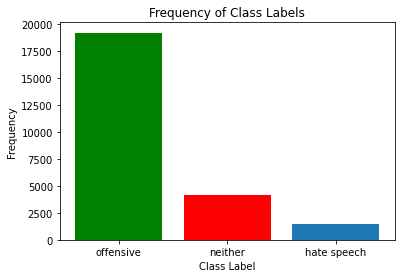
\includegraphics[width=\columnwidth]{Frequency_of_class_labels_in_population}}
\caption{Caption}
\end{figure}

\subsection{Design of Federated Learning System}

We design a single-machine simulation of a Federated Learning system to detect Hate Speech. Figure 2 illustrates the system's architecture. We run an entire Federated Learning system, with one central server and multiple clients on a single machine, using the Flower framework and multiprocessing. Real-world Federated Learning systems must deal with practical issues that are not present in our simulation, such as dynamically changing local datasets, security considerations and connectivity issues (Topal, 2021). Nevertheless, our simulation is a good starting point for evaluating the utility of Federated Learning for hate speech detection.

Our simulation is run in a controlled environment that is suitable for experiments. There is a fixed set of 10 clients, each with a fixed local dataset. The local datasets are formed by partitioning our dataset across the clients. As previously mentioned, for cross-device, supervised Federated Learning tasks, labels should be able to be inferred naturally from user interaction, such as in predictive text (). In hate speech detection, labels can’t be inferred naturally from user interaction. Therefore, supervised approaches to hate speech detection can be federated cross-silo but not cross-device. The Massively Distributed property and the Limited Communication property don't apply to cross-silo Federated Learning, thus they are outside of our scope. In this vein, all clients participate in each round of Federated Learning. We assume a synchronous update scheme that proceeds in rounds of communication. Each round of Federated Learning consists of a training round followed by an evaluation round. There are two main approaches to evaluate models in a Flower federated learning system: centralized evaluation and federated evaluation. In centralized evaluation, the aggregated model is validated on the server-side, and the test set is typically sampled from the original dataset's probability distribution. In federated evaluation, the aggregated model is validated on the client-side, and the test set on each client is sampled from the same probability distribution as the client's training set (Adap GmbH, 2022). We use a federated evaluation approach. The global model is initialized with zeros. At the beginning of each training round, the server sends the current global model parameters to each client. Each client then trains its local model on its local training data, and sends the updated model parameters to the server. The server then aggregates these updates through Federated Averaging and applies them to the global model. At the beginning of each evaluation round, the server sends the current global model parameters to each client. Each client then evaluates the model's validity on its test data, before the whole cycle repeats for 50 rounds.

\begin{figure}[h]
{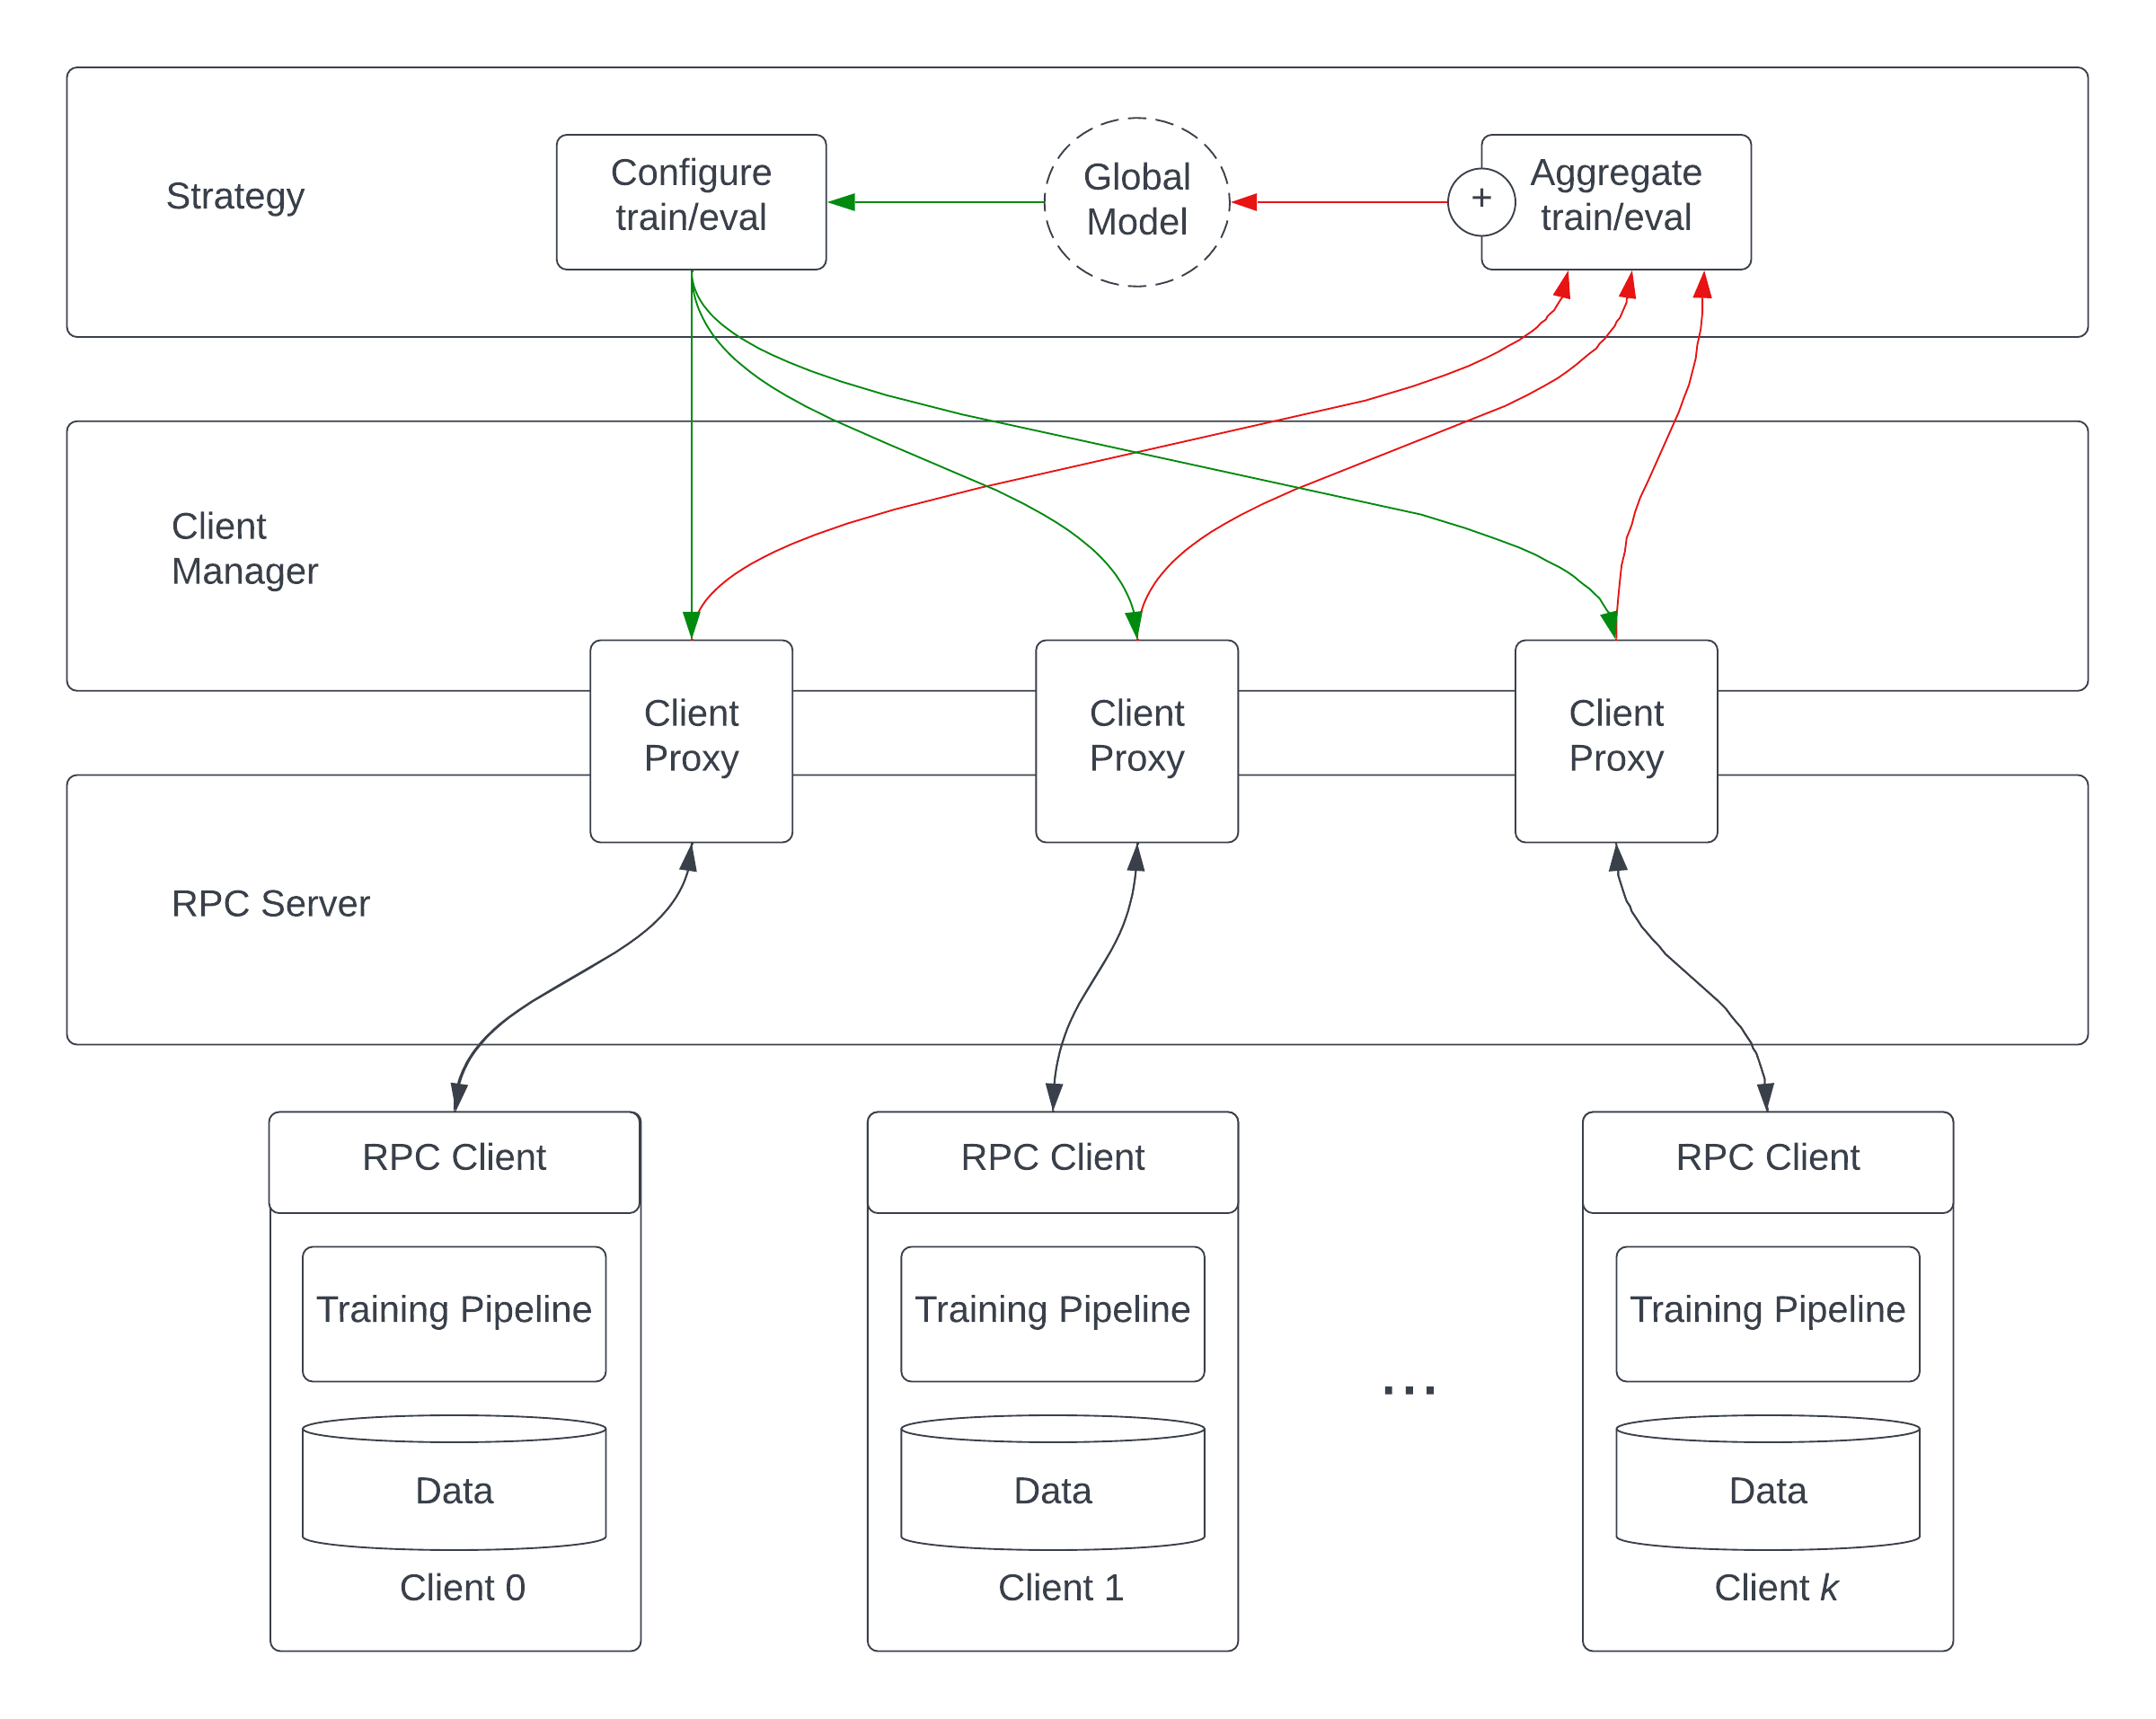
\includegraphics[width=\columnwidth]{High Level Architecture}}
\caption{Caption}
\end{figure}

\subsection{Experimental Design}

In this section, we explain how we assess our proposed Federated Learning System, in terms of its utility. First, we run our simulation under the IID data distribution case as the baseline. We then run the system on the unbalanced and non-IID data distributions characteristic of the federated setting, which existing studies often refer to as the Non-IID setting, as opposed to the IID setting. (Kairouz et al. 2019) gives a taxonomy of unbalanced and non-IID distribution cases. Consider the local discrete probability distribution defined by the joint probability mass function $p^k_{XY}(x_i, y_i)$, where $(x_i, y_i)$ is a sample from our original dataset, with feature vector $x_i$ and label $y_i$. We rewrite $p^k_{XY}(x_i, y_i)$  in terms of the conditional distributions $p^k_{XY}(x_i | y_i)p^k_Y(y_i)$ and $p^k_{XY}(y_i | x_i)p^k_X(x_i)$ to allow us to formalise the 5 cases:
\begin{enumerate}
\item Label Distribution Skew \\ ($\forall{k_1, k_2 \in K}. k_1 \neq k_2 \rightarrow p^{k_1}_Y(y_i) \neq p^{k_2}_Y(y_i)$)
\item Feature Distribution Skew \\ ($\forall{k_1, k_2 \in K}. k_1 \neq k_2 \rightarrow p^{k_1}_X(x_i) \neq p^{k_2}_X(x_i)$)
\item Same labels but different features \\ ($\forall{k_1, k_2 \in K}. k_1 \neq k_2 \rightarrow p^{k_1}_{XY}(x_i | y_i) \neq p^{k_2}_{XY}(x_i | y_i)$)
\item Same features but different labels \\ ($\forall{k_1, k_2 \in K}. k_1 \neq k_2 \rightarrow p^{k_1}_{XY}(y_i | x_i) \neq p^{k_2}_{XY}(y_i | x_i)$)
\item Quantity Skew/Unbalanced data \\ ($\forall{k_1, k_2 \in K}. k_1 \neq k_2 \rightarrow (p^k_{XY}(x_i, y_i) = p^k_{XY}(x_i, y_i) \cap |\mathcal{P}_{k_1}| \neq |\mathcal{P}_{k_2}|)$)
\end{enumerate}
Here, 2. can be simulated by adding varying levels of noise to partitions. In computer vision, these transformations can be done on the fly, using data generators, e.g., for Gaussian noise. However, this isn't the case with NLP. Due to the grammatical structure of the text, a new carefully augmented dataset must be generated beforehand. 3. is mainly relevant to vertical Federated Learning. Similarly to most existing studies, we assume that all clients have the same ground truth, so 4. is irrelevant. Thus, we consider 5. quantity skew and 1. label distribution skew as unbalanced and non-IID distribution cases. To simulate our unbalanced and non-IID distribution cases, we partition our real-world dataset across clients using data partitioning strategies. Many existing studies use the partitioning approach to simulate federated datasets (). To this end, we use the following data partitioning strategies:

\begin{description}
\item[Quantity Skew] We use a Dirichlet distribution to allocate varying amounts of data to each client. We sample $x \sim Dir_K (\beta)$, and allocate a $x_k$ proportion of total data samples to ${\mathcal{P}}_k$ . We fix the distribution parameter, $\beta=10$, to control the degree of imbalance. The smaller $\beta$ is, the more imbalanced the distribution.
\item[Label Distribution Skew: Distribution-based imbalance] Each client is allocated a proportion of the data samples of each label according to a Dirichlet distribution. We sample $p_Y \sim Dir_K(\beta)$ and allocate a $p_{Y,k}$ proportion of the samples labelled $Y$ to client $k$. This partitioning strategy has been used to simulate real world data distributions in recent studies.
\item[Label Distribution Skew: Quantity-based imbalance] Each client owns data samples of a fixed subset of total labels. Such a setting is also used in other studies. We use a general partitioning strategy to set the number of labels that each client has. In the context of our study, this is either 1 or 2. The data samples of each label are split evenly across the clients that have the given label.
\end{description}


During the Federated Learning, we evaluate the convergence behaviour of the global model. In addition, we evaluate the global model's classification metrics, in terms of macro-average precision, recall and f1-score, for comparison against those of local models if the clients were not to participate in our system and remained siloed. There is a class-imbalance in the dataset; the hate speech class and neither class are most important to get right, and they are under-represented. Offensive language class is over-represented. Therefore, macro average is preferable over weighted average, which is misleading in this case (). F1-score is used rather than AUROC because AUROC averages over all possible discrimination thresholds, which is misleading in the case of class-imbalanced data (). In contrast, F1-score maintains a balance between Precision and Recall (). We synthesize 10 samples using each data partitioning strategy. Additionally, we use 10-fold Cross-Validation to randomize the train/test split. Thus, we perform 100 repeats of the simulation per data partitioning strategy and calculate the 95\% Confidence Intervals.
\bigskip
\section{Results}

The Davidson's classifier is a composite classifier that uses 1) Logistic Regression with L1 regularization as a Feature Transformer, to reduce the dimensionality of the data, and 2) Logistic Regression with L2 regularization as a classifier. We use the cross entropy loss function. Recall that any iterative optimization method can be applied to the federated optimization problem. Our system uses one of the most widely used quasi-Newton methods, the Limited-memory Broyden–Fletcher–Goldfarb–Shanno (L-BFGS) algorithm.

\subsection{Convergence of Approach in the Non-IID Setting}

Figure 3 shows the accuracy of the $FedAvg$ approach of our system under different unbalanced and Non-IID data distribution cases. The results for the IID setting are presented as a bench mark. The accuracy does not start at the origin because, as previously mentioned, each evaluation round proceeds a training round in federated evaluation. Therefore, we only evaluate the global model after the first global batch. We constrain the number of local epochs, by dividing the maximum number of iterations that non-federated L-BFGS takes to converge on the full dataset by the number of federated learning rounds. This allows the convergence behaviour of our approach to be observed. The accuracy after the fist training round is noticeably high. If the objective function is non-convex, L-BFGS is not guaranteed to converge. However, if it converges, Newton's Method is much faster than optimization methods such as Gradient Descent. The Cross Entropy loss function is convex. Therefore L-BFGS converges in fewer iterations. From Figure 3 we can observe that, except for the case where each client only has samples of a single class, the $FedAvg$ approach has similar convergence behaviour in the Non-IID setting as in the IID setting. Firstly, for quantity skew, the accuracy is indistinguishable from that for the IID setting. This is down to the fact that $FedAvg$ weighs each client's update with the relative proportion of the client's local dataset. Secondly, in the case of label distribution skew, the algorithm's accuracy for distribution-based label imbalance is similar to that for the IID setting. In the case where clients have samples of two classes, the accuracy is comparable to that for the IID setting; although it varies more across federated learning rounds. On the other-hand the algorithm has the worst accuracy when each client only has samples if a single class.

\subsection{New Heading} 

\begin{figure*}[t]
\resizebox{\textwidth}{!}{
\begin{tabular}{@{}lllll@{}}
\toprule
\textbf{Distribution}     & \multicolumn{2}{c}{Precision (95\% CI)}                           & \multicolumn{2}{c}{Recall (95\% CI)}                              \\ \midrule
                                           & \textbf{Global} & \textbf{Local} & \textbf{Global} & \textbf{Local} \\ \midrule
IID                                        & 0.615 (0.596-0.630)             & 0.579 (0.560-0.597)             & 0.741 (0.701-0.772)             & 0.674 (0.640-0.711)             \\ \midrule
IID Quantity Skew                          & 0.617 (0.598-0.634)             & 0.579 (0.559-0.605)             & 0.742 (0.711-0.771)             & 0.671 (0.643-0.707)             \\ \midrule
Non-IID Distribution Based Label Imbalance & 0.586 (0.545-0.620)             & 0.598 (0.574-0.632)             & 0.722 (0.628-0.770)             & 0.672 (0.635-0.708)             \\ \midrule
Non-IID Quantity Based Label Imbalance 2   & 0.531 (0.477-0.601)             & 0.551 (0.474-0.633)            & 0.697 (0.640-0.766)             & 0.832 (0.787-0.861)              \\ \midrule
Non-IID Quantity Based Label Imbalance 1   & 0.410 (0.358-0.467)             & 0.446 (0.383-0.533)             & 0.733 (0.659-0.800)             & 0.971 (0.956-0.985)             \\ \bottomrule
\end{tabular}
}
\caption{Caption}
\end{figure*}

\begin{figure}[h]
{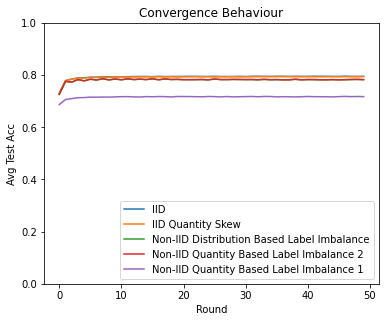
\includegraphics[width=\columnwidth]{Avg_convergence_behaviour}}
\caption{Caption}
\end{figure}

\begin{figure}[h]
{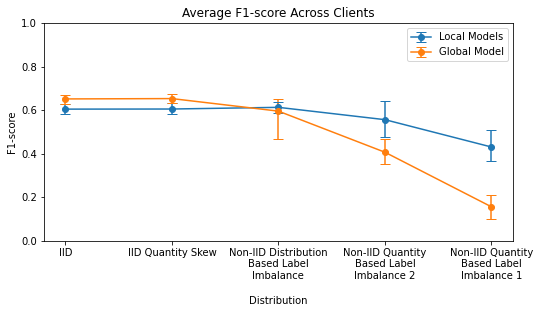
\includegraphics[width=\columnwidth]{Avg_f1_score_of_local_models_against_that_of_global_model}}
\caption{Caption}
\end{figure}

\begin{figure}[h]
{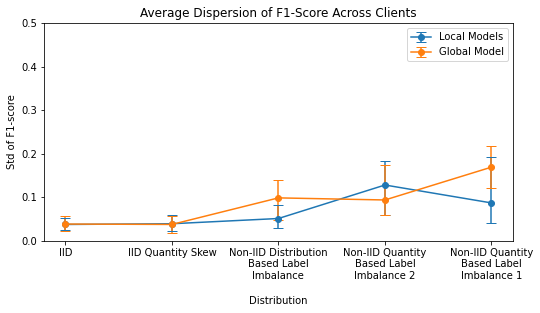
\includegraphics[width=\columnwidth]{Avg_dispersion_of_f1_score_of_local_models_against_that_of_global_model}}
\caption{Caption}
\end{figure}

\bigskip
\section{Discussion}

One reason for the comparable performance of FL might be that
the weight updates and the process of $FedAvg$ could have a similar effect in mini-batches [46-48] and ensembles. In Federated Learning, each client trains on a relatively small dataset and then
sends the local model parameters to the server. The server then aggregates the parameters and updates the global model. Hence, each client is effectively an element of a mini-batch, and the aggregation process is analogous to ensemble processing.

\begin{figure}[h]
{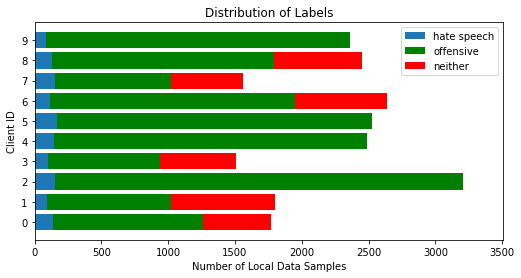
\includegraphics[width=\columnwidth]{noniid-distribution-based-label-imbalance_distribution_of_labels_2}}
\caption{Caption}
\end{figure}

Naive implementations of $FedAvg$ (specifically federated Logistic Regression, sometimes called Homogeneous LR), 'array broadcasts' n dimensional parameters received from certain clients (n is number of labels in the client's sample) to x dimensions, across the array of the client with all labels in the population. Hence suboptimal performance and doesn't work when none of the client samples contain all of the labels in the population.

\begin{figure}[h]
{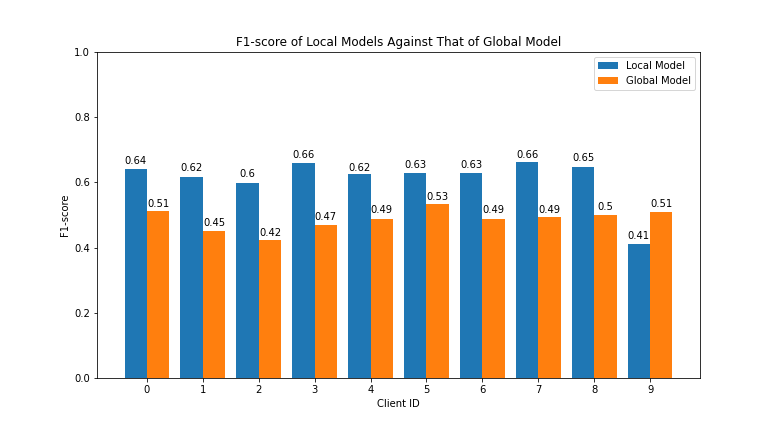
\includegraphics[width=\columnwidth]{noniid-distribution-based-label-imbalance_seed_2performance_of_models_on_client_data_f1score}}
\caption{Caption}
\end{figure}

\subsection{Weight Divergence}

Naively solving an aggregate loss function may implicitly advantage or disadvantage some of the devices, as the learned model becomese biased towards devices with larger amounts of data, or (if weighting devices equally), to commonly occurring groups of devices. 

First wasserstein distance (EMD) between client sample distribution and population distribution can explain why some clients contribute/benefit more than others, link to weight divergence Expand on this...

Recent works have proposed modified modeling approaches that aim to reduce the variance of the model performance across devices. Some heuristics simply perform a varied number of local updates based
on local loss. Other more principled approaches include Agnostic Federated Learning, which optimizes the centralized model for any target distribution formed by a mixture of the client distributions via a minimax optimization scheme. Another more general approach is taken by Li et al., which proposes an objective called q-FFL in which devices with higher loss are given higher relative weight to encourage less variance in the final accuracy distribution.

methods that can work
well with abnormal distributions, robust aggregation, and
efficient communication such as FedProx [16], FSVRG [17],
CO-OP [18], LoAdaBoost FedAVG [19], and RFA [20].
Hyperparameter selection also requires further research.

Move below para elsewhere

A recently emerging technique in the field of natural language processing (NLP) is the employment of transfer learning (Howard and Ruder, 2018; Devlin et al., 2018). The main idea of these approaches is to pretrain a neural language model on large general corpora and then fine-tune this model for a task at hand by adding an additional task-specific layer on top of the language model and training it further. A recent model called Bidirectional encoder representations from transformers (BERT) (Devlinet al., 2018) was pretrained on the concatenation of BooksCorpus (800M words) (Zhu et al., 2015) and English Wikipedia (2,500M words) before being successfully applied to a number of NLP tasks with relatively inexpensive fine-tuning for each task.

\bigskip
\section{Conclusion}
\bigskip

\clearpage
\section{Appendix}

\begin{figure}[hbt!]

\begin{subfigure}{\columnwidth}
{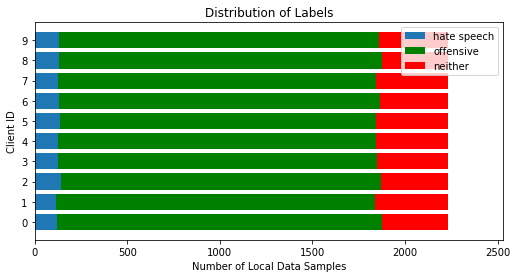
\includegraphics[width=\columnwidth]{iid_distribution_of_labels_7}}
\caption{}
\end{subfigure}%

\begin{subfigure}{\columnwidth}
{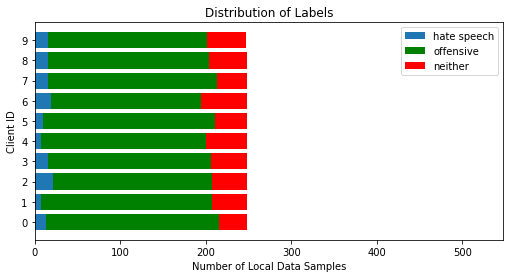
\includegraphics[width=\columnwidth]{iid_test_set_distribution_of_labels_7}}
\caption{}
\end{subfigure}

\caption{}
\end{figure}

\begin{figure}[hbt!]
{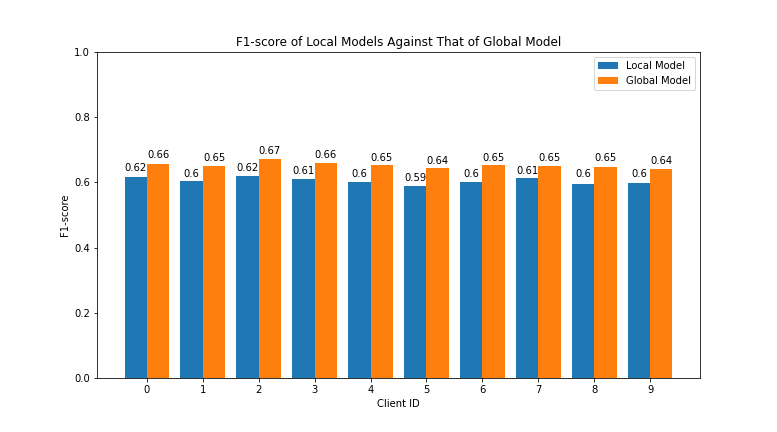
\includegraphics[width=\columnwidth]{iid_seed_7performance_of_models_on_client_data_f1score}}
\caption{}
\end{figure}


\begin{figure}[hbt!]

\begin{subfigure}{\columnwidth}
{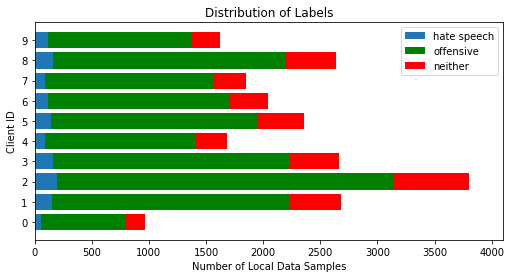
\includegraphics[width=\columnwidth]{iid-quantity-skew_distribution_of_labels_5}}
\caption{}
\end{subfigure}

\begin{subfigure}{\columnwidth}
{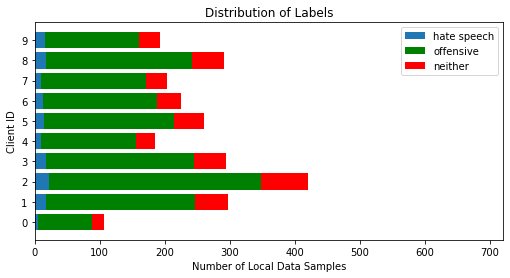
\includegraphics[width=\columnwidth]{iid-quantity-skew_test_set_distribution_of_labels_5}}
\caption{}
\end{subfigure}

\caption{}
\end{figure}

\begin{figure}[hbt!]
{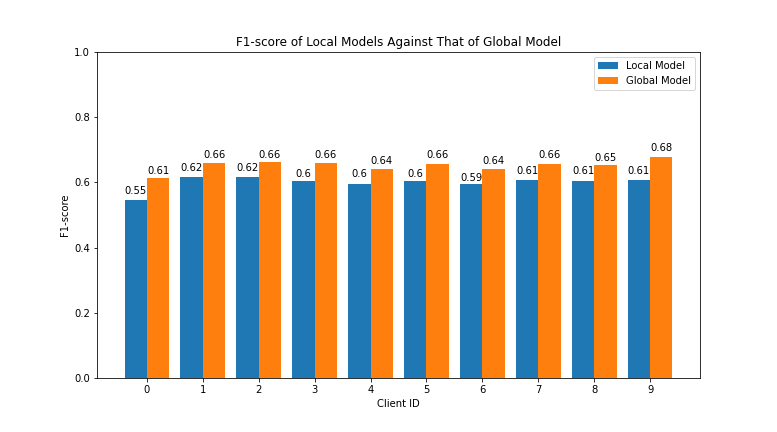
\includegraphics[width=\columnwidth]{iid-quantity-skew_seed_5performance_of_models_on_client_data_f1score}}
\caption{}
\end{figure}


\begin{figure}[hbt!]

\begin{subfigure}{\columnwidth}
{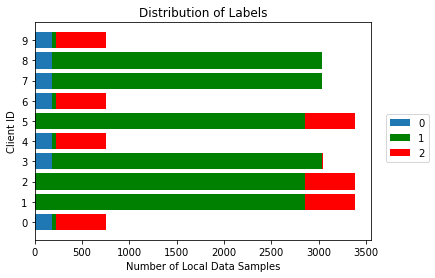
\includegraphics[width=\columnwidth]{noniid-quantity-based-label-imbalance-2_distribution_of_labels_2}}
\caption{}
\end{subfigure}

\begin{subfigure}{\columnwidth}
{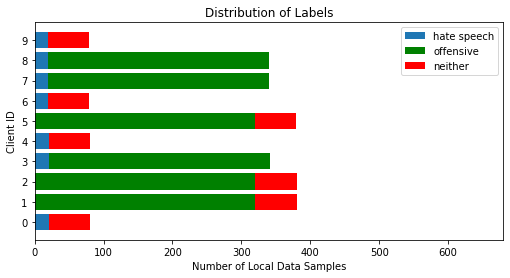
\includegraphics[width=\columnwidth]{noniid-quantity-based-label-imbalance-2_test_set_distribution_of_labels_2}}
\caption{}
\end{subfigure}

\caption{}
\end{figure}

\begin{figure}[hbt!]
{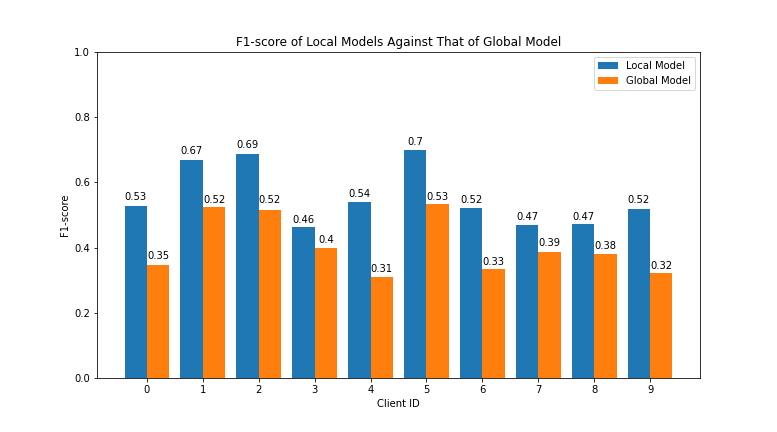
\includegraphics[width=\columnwidth]{noniid-quantity-based-label-imbalance-2_seed_2performance_of_local_models_f1score}}
\caption{Caption}
\end{figure}


\begin{figure}[hbt!]

\begin{subfigure}{\columnwidth}
{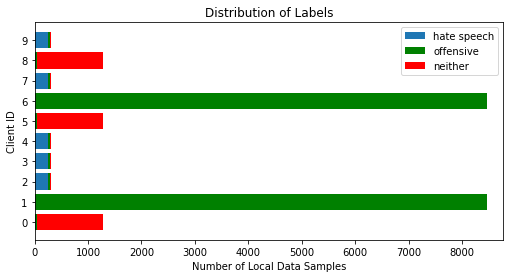
\includegraphics[width=\columnwidth]{noniid-quantity-based-label-imbalance-1_distribution_of_labels_5}}
\caption{Caption}
\end{subfigure}

\begin{subfigure}{\columnwidth}
{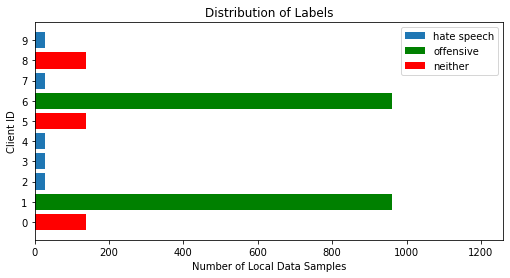
\includegraphics[width=\columnwidth]{noniid-quantity-based-label-imbalance-1_test_set_distribution_of_labels_5}}
\caption{Caption}
\end{subfigure}

\caption{}
\end{figure}

\begin{figure}[hbt!]
{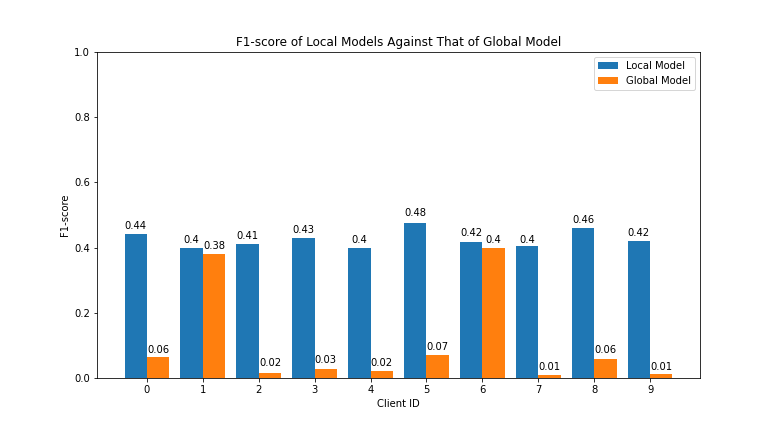
\includegraphics[width=\columnwidth]{noniid-quantity-based-label-imbalance-1_seed_5performance_of_models_on_client_data_f1score}}
\caption{Caption}
\end{figure}


\begin{figure}[hbt!]
{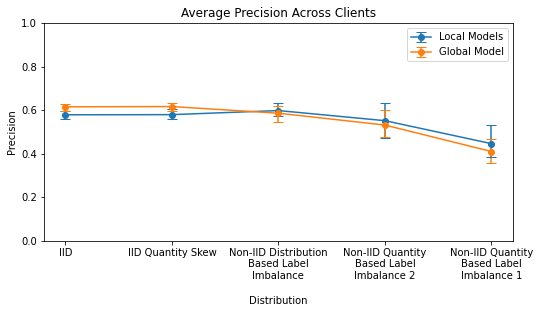
\includegraphics[width=\columnwidth]{Avg_precision_of_local_models_against_that_of_global_model}}
\caption{Caption}
\end{figure}

\begin{figure}[hbt!]
{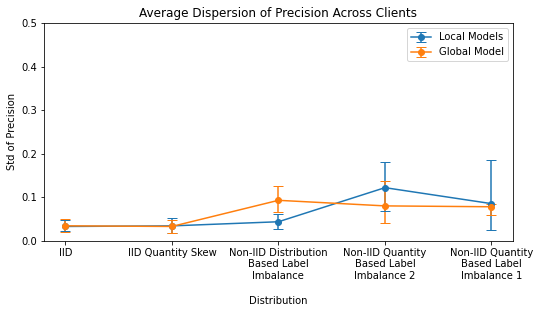
\includegraphics[width=\columnwidth]{Avg_dispersion_of_precision_of_local_models_against_that_of_global_model}}
\caption{Caption}
\end{figure}

\begin{figure}[hbt!]
{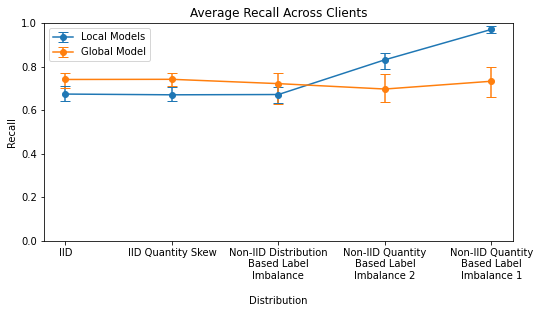
\includegraphics[width=\columnwidth]{Avg_recall_of_local_models_against_that_of_global_model}}
\caption{Caption}
\end{figure}

\begin{figure}[hbt!]
{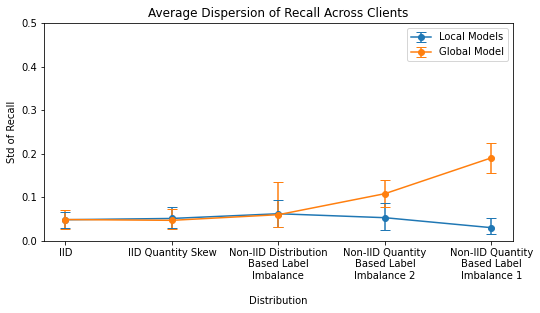
\includegraphics[width=\columnwidth]{Avg_dispersion_of_recall_of_local_models_against_that_of_global_model}}
\caption{Caption}
\end{figure}

\begin{figure*}[t]
\resizebox{\textwidth}{!}{
\begin{tabular}{@{}lllll@{}}
\toprule
\textbf{Distribution}     & \multicolumn{2}{c}{Std of Precision Across Clients (95\% CI)}      & \multicolumn{2}{c}{Std of Recall Across Clients (95\% CI)}         \\ \midrule
                                           & \textbf{Global} & \textbf{Local} & \textbf{Global} & 
                                           \textbf{Local} \\ \midrule
IID                                        & 0.034 (0.019-0.050)              & 0.033 (0.022-0.048)             & 0.048 (0.027-0.069)              & 0.048 (0.030-0.067)             \\ \midrule
IID Quantity Skew                          & 0.033 (0.016-0.048)              & 0.034 (0.018-0.051)             & 0.047 (0.027-0.073)              & 0.051 (0.030-0.077)             \\ \midrule
Non-IID Distribution Based Label Imbalance & 0.093 (0.066-0.125)              & 0.043 (0.026-0.061)             & 0.060 (0.030-0.135)              & 0.062 (0.032-0.093)             \\ \midrule
Non-IID Quantity Based Label Imbalance 2   & 0.080 (0.040-0.136)              & 0.122 (0.067-0.180)            & 0.108 (0.077-0.138)              & 0.053 (0.025-0.087)             \\ \midrule
Non-IID Quantity Based Label Imbalance 1   & 0.078 (0.058-0.083)              & 0.085 (0.024-0.186)             & 0.190 (0.155-0.225)              & 0.030 (0.014-0.053)             \\ \bottomrule
\end{tabular}
}
\caption{Caption}
\end{figure*}

\end{document}
